\documentclass[12pt]{article}

\usepackage[utf8]{inputenc}
\usepackage[english,russian]{babel}
\usepackage{amsmath, amssymb}
\usepackage{graphicx}
\usepackage{epstopdf}

\newcommand{\cutefrac}[2]{{}^{#1\!}\!/{\!}_#2}
\newcommand{\half}{\cutefrac{1}{2}}
\newcommand{\cuteddots}{
\text{
\raisebox{.6ex}{$\cdot$}\hspace{.75em}%
\raisebox{.3ex}{$\cdot$}\hspace{.75em}%
$\cdot$\hspace{.75em}%
\raisebox{-.3ex}{$\cdot$}\hspace{.75em}%
\raisebox{-.6ex}{$\cdot$}%
}}

\graphicspath{{mp/}}

\title{Задание 1}
\date{}

\begin{document}

\maketitle

Мы рассматриваем одномерную задачу о распространении звуковых волн от
гармонического источника на поверхности по неоднородной среде:
\[
\begin{cases}
p_{tt} = c^2(x) p_{xx}\\
p\big|_{t = 0} = 0\\
p_t\big|_{t = 0} = 0\\
p\big|_{x = 0} = \sin \omega t\\
p_t + c(1) p_x \big|_{x = 1} = 0\\
\end{cases},
\]
где $p(t, x)$ --- давление в момент времени $t$ в точке $x$, $\omega$ ---
циклическая частота, с которой воздействуют на поверхность, $c(x)$ --- скорость
звука в точке $x$.

Введем на отрезке $[0, 1]$ сетку с шагом $h = \frac{1}{N}$: 
\[x_i = ih, \quad i =
\overline{0, N}.
\]

Приблизим $p(t, x)$ кусочно-линейной на интервалах $[x_i, x_{i+1}]$ функцией:
\[
p(t, x) = \sum_{i = 0}^N p_i(t) \psi_i(x).
\]
В качестве базисных функций $\psi_i(x)$ возьмем следующие функции:
\begin{figure}[!ht]
\centering
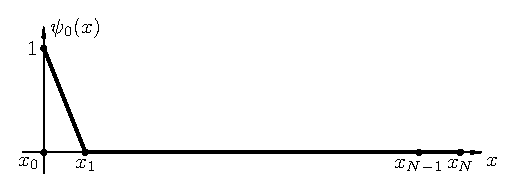
\includegraphics[width=.5\textwidth]{box-0.eps}\\
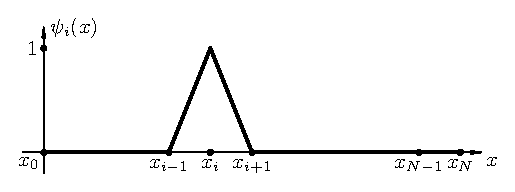
\includegraphics[width=.5\textwidth]{box-1.eps}\\
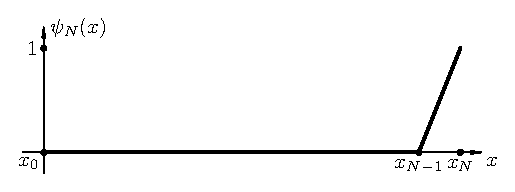
\includegraphics[width=.5\textwidth]{box-2.eps}%
\caption{Базисные функции $\psi_i(t,x)$}
\end{figure}

С такими функциями $\psi_i(x_j) = \delta_{ij}$ и, коэффициенты $p_i(t)$ имеют
смысл значений функции $p(t, x)$ в точках $x = x_i$.

Заметим, что $p_0(t)$ является известной, так как $p_0(t) = p(t, 0) = \sin
\omega t$, поэтому неизвестными являются только $p_1(t), \dots, p_N(t)$.

Чтобы найти приближенное решение задачи, заменим строгое условие
\[
\frac{1}{c^2(x)} p_{tt} - p_{xx} = 0
\]
на более мягкое
\[
\mathcal{G}(p, w) \equiv \int_0^1 \left[\frac{1}{c^2(x)} p_{tt} - p_{xx}\right]
w(x) dx = 0
\]
для всех $w(x)$ из некоторого набора. Заметим, что $w(x)$ входит в функционал
$\mathcal{G}(p, w)$ линейно, то есть, если $\mathcal{G}(p, w_1) = 0$ и
$\mathcal{G}(p, w_2) = 0$, то и $\mathcal{G}(p, \alpha w_1 + \beta w_2) = 0$.
Следовательно, достаточно потребовать, чтобы функционал $\mathcal{G}(p, w)$
обращался в $0$ не для всех $w(x)$ из некоторого семейства функций, а только для
функций $w(x)$ из базиса в этом семействе.

Значение $p$ в точке $x = 0$ зафиксировано. В этом смысле граничные условия
называются жесткими. Напротив, граничные условия в точке $x = 1$ называются
естественными. Эти условия должны быть учтены в функционале $\mathcal{G}(p, w)$.

Для метода Галеркина семейство функций $w(x)$ выбирается из того же класса, что
и класс функций-решений, то есть кусочно-линейных для данного случая. Жесткое
граничное условие налагает на функцию $w(x)$ дополнительное условие $w(0) = 0$.
В некотором смысле, вместо требования выполнения уравнения в точке $x = 0$ мы
требуем выполнение жесткого условия $p(t, 0) = p_0(t)$. Итого, все функции
$w(x)$ представимы в виде $w(x) = \sum_{j=1}^N w_j \psi_j(x)$ (коэффициент при
$\psi_0(x)$ равен $0$). Поскольку $\left\{\psi_j\right\}_{j = 1}^n$ --- базис в
пространстве функций $w(x)$, достаточно потребовать $\mathcal{G}(p, \psi_j) = 0$
для $j = 1, \dots, N$.

\begin{figure}[!ht]
\centering
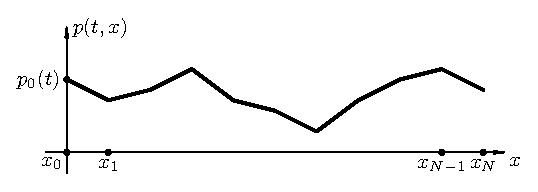
\includegraphics[width=.45\textwidth]{func-0.eps}\quad
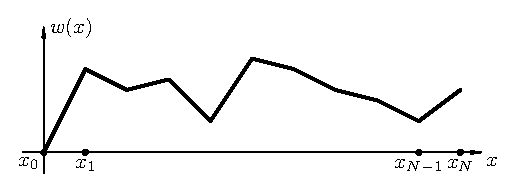
\includegraphics[width=.45\textwidth]{func-1.eps}
\caption{Кусочно линейные функции $p(t,x)$ и $w(x)$}
\end{figure}

Преобразуем выражение для $\mathcal{G}(p, \psi_j) = 0$:
\begin{gather*}
0 = \mathcal{G}(p, w) 
= \int_0^1 \left[\frac{1}{c^2(x)} p_{tt} - p_{xx}\right] w(x) dx = \\
= 
\int_0^1 \frac{p_{tt}(t, x) w(x)}{c^2(x)} dx
-p_{x}(t, x) w(x)\Big|_0^1
+\int_0^1 p_{x}(t, x) w'(x) dx.
\end{gather*}
Учтем граничные условия $w(0) = 0$ и $p_x(t, 1) =
-\displaystyle\frac{1}{c(1)}p_t(t, 1)$:
\begin{gather*}
0 = \mathcal{G}(p, w)
= 
\int_0^1 \frac{p_{tt}(t, x) w(x)}{c^2(x)} dx
+\frac{p_{t}(t, 1) w(1)}{c(1)}
+\int_0^1 p_{x}(t, x) w'(x) dx.
\end{gather*}
Подставляя разложение для $p(t, x)$ и $\psi_j(x)$ вместо $w(x)$, получаем систему
дифференциальных уравнений для $p_i(t)$:
\begin{multline}
0 = \sum_{i=0}^N \ddot p_i(t) \int_0^1 \psi_i(x) \psi_j(x) dx 
+ \sum_{i=0}^N \dot p_i(t) \frac{\psi_i(1) \psi_j(1)}{c(1)} + {}\\
+ \sum_{i=0}^N p_i(t) \int_0^1 \psi_i'(x) \psi_j'(x) dx, \qquad j = 1, \dots,
N.\qquad
\label{eq:ode}
\end{multline}

Для краткости введем несколько обозначений:
\begin{itemize}
\item Матрица масс $M_{ij} = \displaystyle\int_0^1 \frac{\psi_i(x)\psi_j(x)}{c^2(x)} dx$
\item Матрица демпфирования $D_{ij} =
\displaystyle\frac{\psi_i(1)\psi_j(1)}{c(1)}$
\item Матрица жесткости $K_{ij} = \displaystyle\int_0^1 \psi_i'(x)\psi_j'(x) dx$
\end{itemize}
Отметим, что все матрицы оказались симметричными. Обозначим для краткости
$\gamma(x) = \frac{1}{c^2(x)}$. 

Для простоты вычисления матрицы $M$ ограничимся случаем кусочно-постоянной
функции $c(x)$. Пусть значение $c(x)$ на интервале $[x_i, x_{i+1}]$ равно 
$c_{i+\half}$

\begin{figure}[!ht]
\centering
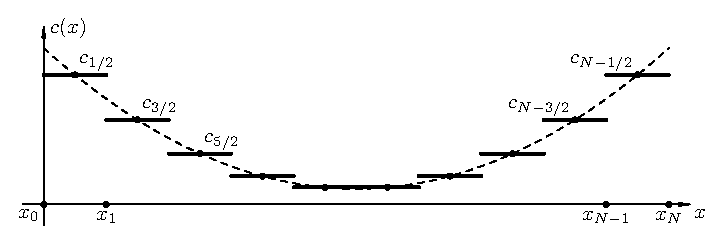
\includegraphics[width=.8\textwidth]{func-2.eps}
\caption{Кусочно постоянная функция $c(x)$}
\end{figure}

Элементы матриц $M_{ij}, D_{ij}$ и $K_{ij}$ равны нулю при $|i - j| > 1$, 
поскольку подынтегральные выражения обращаются в нуль тождественно. Для
остальных элементов верны следующие выражения:
\begin{align*}
M_{00} &= \int_0^1 \gamma(x) \psi_0^2(x) dx = \gamma_{\half}\int_0^h
\left(1-\frac{x}{h}\right)^2 dx = h \gamma_{\half} \int_0^1 (1-\xi)^2 d\xi =
\frac{\gamma_{\half}h}{3}\\
M_{NN} &= \int_0^1 \gamma(x) \psi_N^2(x) dx = \gamma_{N - \half}\int_{1-h}^1
\left(\frac{x + h - 1}{h}\right)^2 dx = h \gamma_{N - \half} \int_0^1 \xi^2 d\xi =
\frac{\gamma_{N - \half}h}{3}\\
M_{ii} &= \int_0^1 \gamma(x) \psi_i^2(x) dx = 
\gamma_{i - \half}\int_{x_{i-1}}^{x_i} \left(\frac{x - x_{i-1}}{h}\right)^2 dx +
\gamma_{i + \half}\int_{x_i}^{x_{i+1}} \left(\frac{x_{i+1} - x}{h}\right)^2 dx =\\ 
&= \frac{(\gamma_{i-\half} + \gamma_{i+\half})h}{3}\\
M_{i,i+1} &= M_{i+1,i} = \int_0^1 \gamma(x) \psi_i(x) \psi_j(x) dx = 
\gamma_{i + \half}\int_{x_i}^{x_{i+1}} 
\left(\frac{x_{i+1} - x}{h}\right)\left(\frac{x - x_i}{h}\right) dx =\\
&= 
\gamma_{i+\half} h \int_0^1 \xi(1-\xi) d\xi = \frac{\gamma_{i+\half}h}{6}
\end{align*}

\[
M = \frac{h}{6}
\begin{pmatrix}
2\gamma_{\half} & \gamma_{\half} & \\
\gamma_{\half} & 2\gamma_{\half} + 2\gamma_{\cutefrac{3}{2}} & \gamma_{\cutefrac{3}{2}}\\
& \gamma_{\cutefrac{3}{2}} & 2\gamma_{\cutefrac{3}{2}} + 2\gamma_{\cutefrac{5}{2}} & \gamma_{\cutefrac{5}{2}}\\
& & \cuteddots\; & \cuteddots & \;\cuteddots \\
& & & \gamma_{N - \cutefrac{3}{2}} & 2\gamma_{N - \cutefrac{3}{2}} + 2\gamma_{N
- \half} & \gamma_{N-\half}\\
& & & & \gamma_{N - \half} & 2\gamma_{N-\half}
\end{pmatrix}
\]

Матрица демпфирования $D$ содержит только один ненулевой элемент:
\[
D_{NN} = \frac{1}{c(1)}
\]

Ненулевые элементы матрицы $K$ равны:
\begin{align*}
K_{00} &= \int_0^1 \left[\psi'_0(x)\right]^2 dx = \int_0^h \frac{1}{h^2} dx =
\frac{1}{h}\\
K_{NN} &= \int_0^1 \left[\psi'_N(x)\right]^2 dx = \frac{1}{h}\\
K_{ii} &= \int_0^1 \left[\psi'_i(x)\right]^2 dx = 
\int_{x_{i-1}}^{x_{i+1}} \frac{1}{h^2} dx = \frac{2}{h}\\
K_{i+1,i} &= K_{i,i+1} = \int_0^1 \psi'_{i}(x) \psi'_{i+1}(x) dx =
\int_{x_i}^{x_{i+1}} \frac{-1}{h^2} dx = -\frac{1}{h}
\end{align*}

\[
K = \frac{1}{h}
\begin{pmatrix}
1 & -1 & \\
-1 & 2 & -1\\
& -1 & 2 & -1\\
& & \ddots & \ddots & \ddots \\
& & & -1 & 2 & -1\\
& & & & -1 & 1
\end{pmatrix}
\]

В данных обозначениях система уравнений \eqref{eq:ode} записывается как:
\[
\sum_{i=0}^N \ddot p_i(t) M_{ij} 
+ \sum_{i=0}^N \dot p_i(t) D_{ij} 
+ \sum_{i=0}^N p_i(t) K_{ij} = 0, \qquad j = 1, \dots,
N.
\]
В этой системе только функции $p_i(t)$ при $i > 0$ являются  неизвестными, в то
время как $p_0(t)$ известна и ее следует исключить из системы уравнений:
\[
\sum_{i=1}^N \ddot p_i(t) M_{ij} 
+ \sum_{i=1}^N \dot p_i(t) D_{ij} 
+ \sum_{i=1}^N p_i(t) K_{ij} = f_j(t), \qquad j = 1, \dots,
N,
\]
где 
\[f_i(t) = -M_{0,i} \ddot p_0(t) -D_{0,i} \dot p_0(t) -K_{0,i} p_0(t).\]

В таком виде, систему можно записать в матричных обозначениях:
\begin{equation}
\ddot{\mathbf{p}}(t) \mathbf{M} + \dot{\mathbf{p}}(t) \mathbf{D}
+ \mathbf{p}(t) \mathbf{K} = \mathbf{f}(t).
\label{eq:vector}
\end{equation}
\begin{gather*}
\mathbf{M} = 
\frac{h}{6}
\begin{pmatrix}
2\gamma_{\half} + 2\gamma_{\cutefrac{3}{2}} & \gamma_{\cutefrac{3}{2}}\\
\gamma_{\cutefrac{3}{2}} & 2\gamma_{\cutefrac{3}{2}} + 2\gamma_{\cutefrac{5}{2}} & \gamma_{\cutefrac{5}{2}}\\
& \cuteddots\; & \cuteddots & \;\cuteddots \\
& & \gamma_{N - \cutefrac{3}{2}} & 2\gamma_{N - \cutefrac{3}{2}} + 2\gamma_{N
- \half} & \gamma_{N-\half}\\
& & & \gamma_{N - \half} & 2\gamma_{N-\half}
\end{pmatrix}
\\
\mathbf{K} = 
\frac{1}{h}
\begin{pmatrix}
2 & -1\\
-1 & 2 & -1\\
& \ddots & \ddots & \ddots \\
& & -1 & 2 & -1\\
& & & -1 & 1
\end{pmatrix}\qquad
\mathbf{D} = 
\begin{pmatrix}
0  \\
& 0 \\
& & \ddots \\
& & & 0 \\
& & & & \frac{1}{c(1)}
\end{pmatrix}
\end{gather*}
Здесь $\mathbf{M}, \mathbf{D}$ и $\mathbf{K}$ --- подматрицы матриц $M, D$ и
$K$, но без нулевой строки и нулевого столбца, а $\mathbf{p}(t)$ --- вектор-строка из 
функций $p_1(t), \dots, p_N(t)$. Вектор $\mathbf{f}(t)$ имеет вид
\[
\mathbf{f}(t) = 
\begin{pmatrix}
-M_{0,1}\omega^2 \sin \omega t + \dfrac{1}{h} \sin \omega t & \quad 0 \quad & \cdots & \quad 0
\end{pmatrix}
\]

Система \eqref{eq:vector} не разрешена относительно старшей производной
$\ddot{\mathbf{p}}(t)$, а вычислять обратную матрицу $\mathbf{M}^{-1}$ или
решать линейную систему на каждом временном шаге оказывается слишком трудоемко
на практике. Вместо этого, пытаются модифицировать метод так, чтобы матрица
$\mathbf{M}$ получилась диагональной.

Простейший способ получить такой метод --- изменить процедуру вычисления
элементов матриц $M$ и $K$, заменив точное интегрирование на интегрирование
методом трапеций (матрица $K$ при этом не меняется):
\begin{align*}
&\quad\int_{x_i}^{x_{i+1}} f(x) dx \approx h\frac{f(x_i) + f(x_{i+1})}{2}\\
\widetilde{M}_{00} &= \int_0^1 \gamma(x) \psi_0^2(x) dx 
= h \gamma_{\half} \int_0^1 (1-\xi)^2 d\xi \approx
\frac{\gamma_{\half}h}{2}\\
\widetilde{M}_{NN} &= \int_0^1 \gamma(x) \psi_N^2(x) dx
= h \gamma_{N - \half} \int_0^1 \xi^2 d\xi \approx
\frac{\gamma_{N - \half}h}{2}\\
\widetilde{M}_{ii} &= \int_0^1 \gamma(x) \psi_i^2(x) dx \approx 
\frac{(\gamma_{i-\half} + \gamma_{i+\half})h}{2}\\
\widetilde{M}_{i,i+1} &= \widetilde{M}_{i+1,i} = \int_0^1 \gamma(x) \psi_i(x) \psi_j(x) dx
= \gamma_{i+\half} h \int_0^1 \xi(1-\xi) d\xi \approx 0\\
\widetilde{\mathbf{f}}(t) &= 
\begin{pmatrix}
\dfrac{1}{h} \sin \omega t & \quad 0 \quad & \cdots & \quad 0
\end{pmatrix}
\end{align*}

\begin{gather*}
\widetilde{M} = \frac{h}{2}
\begin{pmatrix}
\gamma_{\half} & \\
& \gamma_{\half} + \gamma_{\cutefrac{3}{2}}\\
& & \gamma_{\cutefrac{3}{2}} + \gamma_{\cutefrac{5}{2}}\\
& & & \ddots \\
& & & & \gamma_{N - \cutefrac{3}{2}} + \gamma_{N - \half}\\
& & & & & \gamma_{N-\half}
\end{pmatrix}
\\
\widetilde{\mathbf{M}} = \frac{h}{2}
\begin{pmatrix}
\gamma_{\half} + \gamma_{\cutefrac{3}{2}}\\
& \gamma_{\cutefrac{3}{2}} + \gamma_{\cutefrac{5}{2}}\\
& & \ddots \\
& & & \gamma_{N - \cutefrac{3}{2}} + \gamma_{N - \half}\\
& & & & \gamma_{N-\half}
\end{pmatrix}
\end{gather*}
Ту же матрицу можно получить просуммировав в каждой строке $M$ элементы и поместив
сумму на диагональ. Система обыкновенных дифференциальных уравнений теперь
тривиально разрешается относительно старшей производной, поскольку матрица
$\widetilde{\mathbf{M}}$ диагональна.
\begin{equation}
\ddot{\mathbf{p}}(t) \widetilde{\mathbf{M}} + \dot{\mathbf{p}}(t) \mathbf{D}
+ \mathbf{p}(t) \mathbf{K} = \widetilde{\mathbf{f}}(t).
\label{eq:vector2}
\end{equation}
Дискретизируем временные производные стандартным образом:
\begin{equation}
\frac{\mathbf{p}^{n+1} -2 \mathbf{p}^n + \mathbf{p}^{n-1}}{\tau^2}
\widetilde{\mathbf{M}}
+
\frac{\mathbf{p}^{n+1} - \mathbf{p}^{n-1}}{2\tau}
\mathbf{D}
+
\mathbf{p}^n \mathbf{K} = \widetilde{\mathbf{f}}^n.
\label{eq:difference}
\end{equation}
Здесь верхний индекс означает номер шага по времени. Перепишем разностную задачу
в разрешенном относительно $\mathbf{p}^{n+1}$ виде:
\begin{equation}
\mathbf{p}^{n+1} \left(
\widetilde{\mathbf{M}} + \frac{\tau}{2} \mathbf{D}
\right)
+
\mathbf{p}^{n-1} \left(
\widetilde{\mathbf{M}} - \frac{\tau}{2} \mathbf{D}
\right)
+
\mathbf{p}^n \left(
\tau^2\mathbf{K}-2\widetilde{\mathbf{M}}
\right)
 = \tau^2\widetilde{\mathbf{f}}^n.
\label{eq:difference2}
\end{equation}
В качестве начальных данных для \eqref{eq:difference2} можно задать
$\mathbf{p}^0 = \mathbf{p}^1 = 0$, что соответствует начальным данным для
исходной задачи. 

\emph{Задание}. Запрограммировать метод \eqref{eq:difference2} с параметрами 
$\omega = 5$, числом интервалов $N = 200$, шагом по времени $\tau = \frac{h}{2}$
и решить задачу до момента времени $t_{\max} = 10$. Скорость звука зависит от
координаты по следующему закону:
\[
c_{i+\half} = c\left( (i + \half) h\right), \qquad c(x) = 0.1 + 3.6 (x - 0.5)^2.
\]
В качестве результатов необходимо прислать график $p(t, x)$ в момент времени $t =
t_{\max}$ и исходный код программы.

\end{document}
